% A presentation of the theoretical background necessary to understand your project. Not every project will need a theory section, but most will. Here you would describe the physics of how sensors you use work (eg how does accelerometer measure acceleration, or how does a capacitive touch sensor work), or how an electrical interface to a device works.

\subsection{Digital - Analog Converter}\label{subsec:digital---analog-converter}

The primary goal of a digital to analog converter is to convert data bits (strictly HIGH or LOW), and convert to an analog signal with voltage varying on the values of the data bits.
This can be done either by receiving all data pins at once, or sending the data pins individually along with a clock bit, which is then read by a segment in the integrated circuit that decodes the data.
Receiving all data pins at once does not require the use of an integrated circuit, and can be done using resistor ladders.
More details regarding resistor ladders will be shown below.
Nonetheless, the DAC allows us to input a certain number of bits, in the case of this project, 10 bits, and convert to an analog signal (thereby giving us 1024 different values from 0 volts up until the maximum voltage).
This is essentially "receiving what output voltage to emit in binary", so that 1111111111, all pins on, corresponds to the maximum voltage, and 0000000000 (all pins off) correspond to minimum voltage, and something like 1101100110 till be $\frac{870}{1023}$ of the maximum. 

\subsection{Analog - Digital Converter}\label{subsec:analog---digital-converter}

an analog to digital works in the exact opposite way as a digital to analog converter.
By taking in an input voltage (as a proportion of the maximum voltage), an analog to digital converter will set some data value to be equal to that input voltage as a binary proportion to the maximum (or reference) voltage.
In the case of the microprocessor, this will be 3.3 volts.
The usage of this in the project is to be able to perform certain actions based on the value of this input pin, i.e. control the frequency based on what notes are being pressed. 

\subsection{Low Pass Filter}\label{subsec:low-pass-filter}

The theory behind an analog low pass filter is relatively simple;
the signal is sent through an RC circuit (see figure~\ref{fig:LPF}), which, due to the charging and discharging properties of a capacitor, allows us to block frequencies past a certain cutoff frequency.
This cutoff frequency is given by the following formula:

\[
f_{cutoff}=\frac{1}{2 \pi R C}
\]

So, in order to reduce unnecessary signal noise, we can apply a low pass filter to block frequencies past the human range of hearing, as well as attenuate higher pitched distortion coming from the circuit. 

In the specific case of this project, a 9.55 nF capacitor was made available.
Using the formula mentioned above, we can set the cutoff frequency to 20 kHz, therefore using a resistor of 800 Ohms. 

\begin{figure}[H]
    \centering
    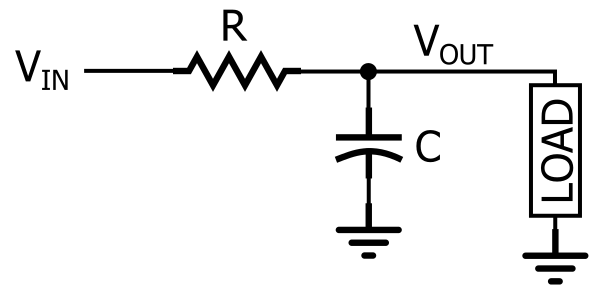
\includegraphics[width = 0.4 \textwidth]{lowpassfilter}
    \caption{A basic circuit diagram of a low pass filter. } % cite here
    % https://www.allaboutcircuits.com/technical-articles/low-pass-filter-tutorial-basics-passive-RC-filter/
    \label{fig:LPF}
\end{figure}

We can graph what the resultant signal graph will be post-LPF by using the following formula. This formula is derived from the formula for a voltage divider circuit. 



\[
V_{out}=V_{in}\left(\frac{X_{C}}{\sqrt{R_{1}^{2}+X_{C}^{2}}}\right)
\]

where

\[
X_{C}=\frac{1}{2 \pi f C}
\]

Hence, assuming $V_{in}$ is kept constant at 3.3 volts, we can view the output voltage as a function of the frequency, with $C = 9.55*10^{-9}$ F, and $R_1 = 800 \Omega$. 

\begin{figure}[H]
    \centering
    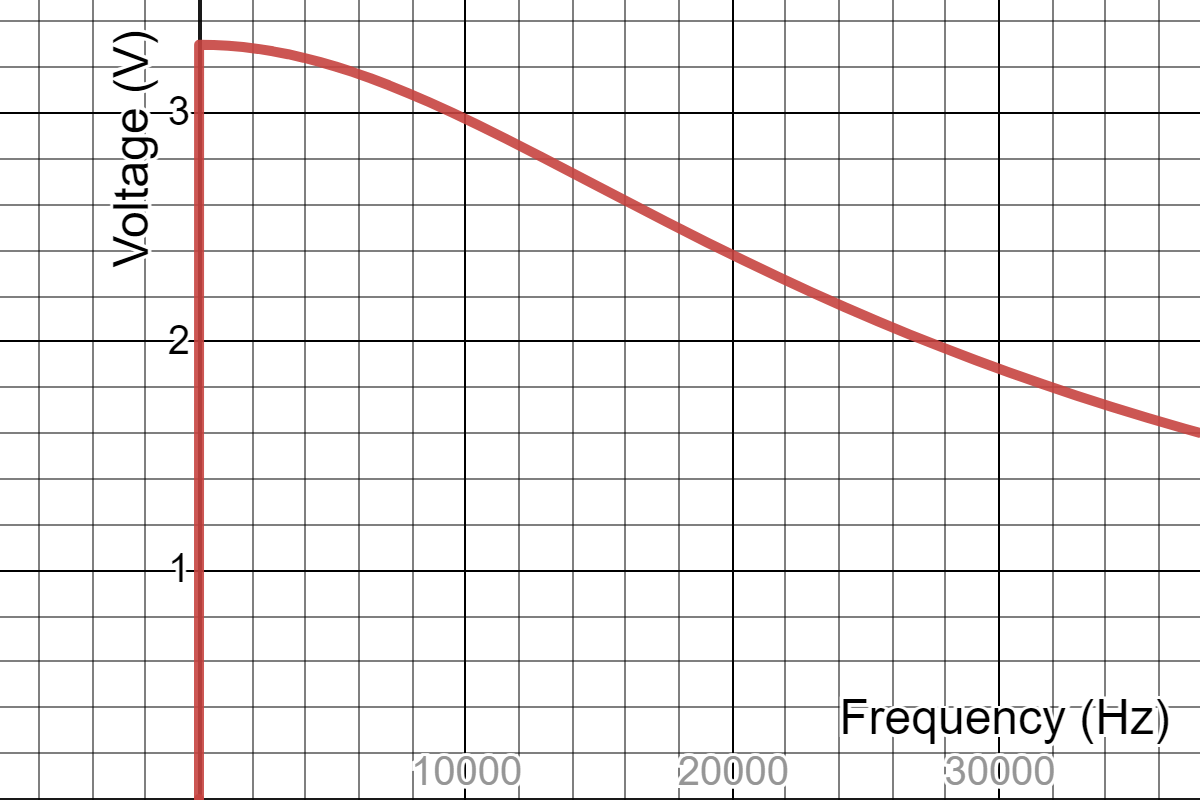
\includegraphics[width = 0.5 \textwidth]{lpfgraph}
    \caption{Plot of voltage versus frequency (linear scale) for an RC low pass filter. }
    \label{fig:lpfgraph}
\end{figure}

\subsection{MIDI Standard}\label{subsec:midi-standard-theory}
% https://www.instructables.com/Send-and-Receive-MIDI-with-Arduino/

Next, we delve further into details regarding the MIDI standard.
Note that this is strictly regarding the standard, and details regarding receiving MIDI data on the microprocessor will be described in Section~\ref{subsec:previous-apparatus-renditions}.

Sending MIDI data works by sending a stream of bytes at a given baud rate\footnote{The rate at which information is transferred in a communication channel.}. %https://www.setra.com/blog/what-is-baud-rate-and-what-cable-length-is-required-1#:~:text=The%20baud%20rate%20is%20the,of%209600%20bits%20per%20second.
This data is then decoded and processed, and instrument-related actions are taken accordingly. 

MIDI data is sent in either 2 or 3 bytes of information, depending on what the first byte is.
The first byte is always a command byte:

\[
\begin{array}{l|l}
10000001 & \text { note off } \\
10010001 & \text { note on } \\
10100001 & \text { aftertouch } \\
10110001 & \text { continuous controller } \\
11000001 & \text { patch change } \\
11010001 & \text { channel pressure } \\
11100001 & \text { pitch bend } \\
11110001 & \text { non-musical commands }
\end{array}
\]

The latter half-byte in the command is what channel the command is being sent on (in this case, they are all being sent on channel 1. 

If the command is a Note On, Note Off, or aftertouch, the first byte that is sent after the command is what note was pressed, and the second is the velocity value or aftertouch value, respectively. IF the command is a controlled change or similar, the first byte that is sent after the command is what controller number was changed, and its new value. We are ignoring aftertouch, patch change, channel pressure, pitch bend, and non-musical commands in this project. 

Hence, we can read the first byte, quickly decode it, and read the second byte and third byte accordingly.
The C implementations are in Appendix~\ref{sec:-table-of-notes-to-frequency-values}.

When reading a note on / off command, the second byte corresponds to what note is being played.
There is a direct conversion from the MIDI note to the frequency, through the following formula:




\subsection{PWM-Based Synthesis}\label{subsec:pwm-based-synthesis-theory}

\subsection{Envelope Generation}\label{subsec:envelope-generation-theory}